\section{Experimentación y resultados}


\textbf{En la tabla \ref{tab:res_exp} se muestra un esquema de los optimizadores, modelos y conjuntos de datos utilizados en cada experimento.}


\begin{table}[H]
\centering
\renewcommand{\arraystretch}{1.2} % Ajusta el espaciado entre filas
\resizebox{\textwidth}{!}{\begin{tabular}{|p{3.5cm}|p{3.5cm}|p{4.5cm}|p{3.5cm}|}
\hline
\textbf{Experimentos} & \textbf{Optimizadores} & \textbf{Conjuntos de datos} & \textbf{Modelos} \\ \hline
1. Diferencia del rendimiento según la tarea & 
SHADE, SHADE-ILS, AdamW, RMSProp & 
BCW, BHP, WQR, WQC & 
MLP \\ \hline

2. Impacto de factores en el rendimiento & 
SHADE, SHADE-ILS, AdamW, RMSProp & 
BCW, WQC, MNIST, F-MNIST, CIFAR-10G & 
MLP, LeNet5, ResNet15, ResNet57 \\ \hline

3. Análisis de tiempos de ejecución & 
SHADE-ILS, SHADE, AdamW & 
\raggedright BCW, BHP, WQR, WQC, MNIST, F-MNIST, CIFAR-10G & 
MLP, LeNet5, ResNet15, ResNet57 \\ \hline

4. Evaluación de propuestas propias & 
\raggedright SHADE, SHADE-ILS, SHADE-GD, SHADE-ILS-GD & 
\raggedright BCW, BHP, WQR, WQC, MNIST, F-MNIST, CIFAR-10G & 
MLP, LeNet5, ResNet15, ResNet57 \\ \hline
\end{tabular}}
\caption[Descripción de los experimentos realizados, optimizadores evaluados, conjuntos de datos utilizados y modelos empleados en el estudio]{Descripción de los experimentos realizados, optimizadores evaluados, conjuntos de datos utilizados y modelos empleados en el estudio. El Experimento 1 compara el rendimiento los optimizadores MH SHADE y SHADE-ILS en relación al de los basados en gradiente AdamW y RMSProp, comprobando si existen diferencias en el rendimiento relativo según el tipo de tarea. En el Experimento 2, se analiza el impacto de diversos factores en el rendimiento de los algoritmos, empleando AdamW y RMSProp como representantes de GD y SHADE y SHADE-ILS como MH. El Experimento 3 evalúa los tiempos de ejecución de los optimizadores en distintos conjuntos de datos y modelos. SHADE se analiza de manera implícita, ya que constituye el núcleo del algoritmo SHADE-ILS. Finalmente, en el Experimento 4, se comparan las propuestas SHADE-GD y SHADE-ILS-GD con sus versiones originales, para posteriormente compararlas entre ellas. Se elige los optimizadores basados en GD AdamW y RMSProp ya que son los que mejores resultados obtienen en la experimentación de manera genreal. Adicionalmente, se emplean estos dos junto con los optimizadores Adam y NAG en pruebas preliminares para determinar cuál de ellos ofrece el mejor desempeño en cada tarea. Este análisis permite integrar el optimizador GD más adecuado dentro de SHADE-GD y SHADE-ILS-GD, maximizando así su eficiencia en cada contexto.}
\label{tab:res_exp}
\end{table}


\subsection{Entorno de ejecución y detalles de implementación}

En esta sección se detallará el entorno de pruebas junto con las justificaciones de las elecciones realizadas a lo largo de la experimentación. Para el desarrollo del código se usa el lenguaje Python principalmente con las librerías PyTorch, FastAI, Numpy, SKlearn y Pandas; implementado y ejecutado en la plataforma Paperspace, que proporciona un IDE y un entorno de ejecución online similar a Google Colab, pero en el que podemos elegir manualmente el hardware sobre el que ejecutamos el código, de manera que la comparación de tiempos y recursos entre las distintas técnicas sea objetiva. 

 Las librerías utilizadas son: FastAI 2.7.17, NBdev 2.3.31, Ucimlrepo 0.0.7, Torchvision 0.16.1+cu121, Matplotlib 3.7.3, Scikit-learn 1.3.0, Scipy 1.11.2, Torch 2.1.1+cu121, Numpy 1.26.3, Pandas 2.2.0 y Pyade 1.0. El hardware usado es Nvidia Quadro P5000, proporcionado por la plataforma. El código puede encontrarse en: \url{https://github.com/eedduu/TFG}. 

Dada la cantidad de modelos distintos que vamos a entrenar, se ha decidido dividir el código en un archivo por tarea, teniendo cada conjunto de datos su propio archivo \verb|conjunto_de_datos.ipynb|. Se ha elegido este formato de archivo en lugar de \verb|conjunto_de_datos.py| de manera que se puedan comprobar las salidas del proyecto fácilmente. 

Se ha creado un módulo de python llamado \verb|utilsTFG.py| que contiene funciones comunes al código, como métricas de error propias, herramientas para el preprocesado de datos, los modelos ConvNets, funciones para graficar resultados o los algoritmos MH. También hay un archivo \verb|comparative.ipynb| donde se realizan comparativas a posteriori de los resultados, como por ejemplo graficar relaciones entre los rendimientos de algunas técnicas o llevar a cabo test estadísticos.


En todas las funciones y librerías usadas en las que intervienen generación de números aleatorios se fija el valor de su semilla a 42. Esto se hace al iniciarse el proyecto, de manera que afecte a la separación de los datos en entrenamiento, de test y a la generación de parámetros iniciales para los modelos que vamos a entrenar con GD. Luego se vuelve a fijar la semilla para todas las librerías que corresponda para generar la población que usaremos con las técnicas MH y se fija también de nuevo antes de iniciar cada entrenamiento, de manera que se puedan repetir los experimentos por separado.

Esto último también se realiza ya que la experimentación ha debido realizarse en ejecuciones separadas, y fijando la semilla de nuevo obtenemos el mismo estado para los generadores de números aleatorios, con lo que no tenemos problema al dividir las ejecuciones. Se han guardado además, a través de la librería \verb|pickle|, tanto las poblaciones iniciales como los modelos y tiempos obtenidos para cada tarea, de manera que estos son comprobables.




\subsubsection{Gradiente descendente}

El criterio para elegir los optimizadores basados en GD ha sido el siguiente: en primer lugar decidimos incorporar tres técnicas basadas en GD para tener diversidad en los resultados, como se expone arriba, y en concreto ese es el número de estrategias distintas en los que se dividen a grandes rasgos los optimizadores de primer orden (ver Sección \ref{sec:gd}). Para cada enfoque distinto, seleccionamos el optimizador en función del número de citas de su publicación, su uso en la literatura y su estandarización en librerías de aprendizaje automático. Por tanto hemos elegido \textbf{NAG, RMSProp, Adam y AdamW.}

Entrenamos usando la política de un ciclo de Leslie para alcanzar una convergencia más rápida. Para elegir el valor máximo de la tasa de aprendizaje usamos la función \verb|lr_find()| de FastAI, opción usada ampliamente en la literatura. Hay que destacar que tres de los cuatro optimizadores que usamos tienen tasas de aprendizaje adaptativas, por lo que la elección de la tasa de aprendizaje es notablemente menos influyente en ellos. 

Usamos 20 épocas para el entrenamiento de los modelos con estos optimizadores, valor obtenido del artículo comentado y comprobado experimentalmente que permite la convergencia en todos los entrenamientos. Durante el entrenamiento, guardamos los parámetros del mejor modelo en términos de error de validación, que será el que usemos para calcular el error de generalización y realizar las comparativas.




\subsubsection{Metaheurísticas}

Las principales librerías de aprendizaje automático no incluyen herramientas para entrenar a través de técnicas metaheurísticas ni para manejar los modelos usando estas técnicas, por lo que debemos realizar ciertas implementaciones que nos permitan integrarlas. 

El algoritmo de SHADE se implementa a través de pyade\footnote{\url{https://github.com/xKuZz/pyade/tree/master}}, una librería de Python que nos permite usar varios algoritmos basados en DE controlando sus parámetros. Se le han realizado modificaciones para mantener los parámetros adaptativos del algoritmo SHADE entre ejecuciones distintas y adaptar las estructuras de datos a las del resto del código.

Dicho algoritmo optimiza un vector de valores flotantes, por lo que debemos crear las funciones necesarias para obtener los parámetros de un modelo en forma de array y luego volverlos a cargar en el modelo respetando la estructura por capas del mismo. Además se han creado funciones de coste que funcionan igual que las implementadas por FastAI, ya que están basadas en ellas, pero que manejan la estructura de datos que tenemos que usar con estos algoritmos. Dichas funciones permiten evaluar sobre el conjunto de entrenamiento, validación o test según corresponda. 

A partir del algoritmo SHADE se implementan manualmente el resto. Para la búsqueda local L-BFGS que se usa en SHADE-ILS y SHADE-ILS-GD usamos la función que ofrece la librería Scipy. Como función de error en dicha búsqueda realizamos una modificación de la función de error antes mencionada para que devuelva además el gradiente, necesario para dicho algoritmo. Para los algoritmos meméticos, a la hora de realizar el entrenamiento a través de GD, simplemente usamos las funciones mencionadas anteriormente para cargar los pesos en un objeto \verb|learner| de FastAI y entrenar una época, para después devolver los pesos actualizados a la estructura de datos necesaria.

Cuando entrenamos los modelos usando técnicas MH tenemos que asignar muchos más recursos al entrenamiento si queremos alcanzar unos resultados parecidos. Una época ocurre cada vez que evaluamos el conjunto de entrenamiento entero con la función de pérdida. Utilizando 20 épocas para el entrenamiento de nuestros modelos no ocurren apenas mejoras, obteniendo un resultado equiparable al que conseguimos con las inicializaciones aleatorias de pesos, ya que en el algoritmo SHADE en cada generación tenemos que evaluar el modelo sobre el conjunto de entrenamiento un total de $N_{pob}$ veces. Con los valores usados el algoritmo solo ejecutaría dos generaciones, una cifra insignificante en este aspecto.

Para que el entrenamiento pueda ser comparable y se siga un criterio claro a la hora de asignar recursos, vamos a redefinir el concepto de época para el entrenamiento con estos algoritmos. Siguiendo el criterio establecido en \cite{MHtrainingClase} y usando como referencia el algoritmo SHADE-ILS, vamos a establecer que una época realiza un total de 210 evaluaciones sobre el conjunto de entrenamiento. Esto surge de utilizar 200 evaluaciones para el algoritmo SHADE y 10 para el algoritmo de búsqueda local. Así, al entrenar 20 épocas, tendríamos un total de 4200 evaluaciones sobre el conjunto de entrenamiento, mientras que los optimizadores realizarían 20. En el caso de ejecutar SHADE, otorgamos esas 10 evaluaciones pertenecientes a la búsqueda local también al algoritmo poblacional.

En los algoritmos meméticos, la ejecución del GD se realiza cada dos épocas, es decir cada 420 evaluaciones. Por tanto aunque contamos las evaluaciones realizadas por el optimizador que corresponda, a efectos prácticos no restarían ejecuciones ni a la búsqueda local ni al algoritmo generacional ya que la comprobación de que se ha superado el número máximo de evaluaciones se realiza siempre al final de la generación.

Durante el entrenamiento con las técnicas MH se evalúan los modelos únicamente sobre el conjunto de entrenamiento, guardando un array con el mejor modelo hasta esa generación y su correspondiente error. Luego, se evalúa cada modelo del array sobre el conjunto de validación y se selecciona el que menor error tenga sobre él de cara a calcular el error de generalización y comparar con el resto de técnicas. De esta manera establecemos un criterio similar al que usamos para seleccionar el mejor modelo entrenado con un optimizador basado en GD.

En las técnicas meméticas, a la hora de entrenar una época con GD no usamos la política de ciclos de Leslie. En primer lugar porque no está diseñada para entrenamientos tan cortos y no sería efectiva. En segundo lugar el uso de tasas de aprendizaje que aumenten hasta valores altos tiene un objetivo exploratorio del paisaje de la función de coste, elemento que ya tenemos gracias a la parte basada en poblaciones del algoritmo memético, por lo que nos interesa centrarnos más en la explotación de una buena región de dicho paisaje.


\subsubsection{Entrenamiento}

Usamos los cuatro optimizadores de primer orden basados en GD mencionados anteriormente con un doble objetivo. En primer lugar así tenemos resultados más diversos con los que comparar las técnicas MH, pudiendo observar si estos algoritmos mejoran a alguno o ninguno de los optimizadores propuestos. Como los cuatro optimizadores son ampliamente usados en la literatura, creemos que esta información es pertinente. Por otro lado, sabemos que el optimizador que mejores resultados consiga depende ampliamente de la tarea y del modelo, por tanto, al ejecutar las técnicas hibridadas con el GD podemos asignar a cada modelo el optimizador que mejor rendimiento haya ofrecido en la tarea.

En las estrategias MH elegimos usar SHADE y SHADE-ILS. El primero es uno de los algoritmos sin búsqueda local que mejores resultados ofrece en optimización de problemas continuos, mientras que el segundo es un referente en la optimización de problemas continuos a gran escala y especialmente en el entrenamiento de modelos. Además proponemos dos técnicas nuevas: SHADE-GD y SHADE-ILS-GD, que resultan de la hibridación de las anteriores con el GD. 

Debido a la sensibilidad del entrenamiento a los parámetros iniciales, se han usado los mismos pesos iniciales para los entrenamientos con distintos optimizadores de un mismo modelo. De manera similar, se usa la misma población inicial de soluciones para un mismo modelo en cada entrenamiento con técnicas MH. Se ha usado la inicialización de pesos Glorot, al igual que en el paper de referencia. Como diferencia respecto a dicha publicación, no usamos validación cruzada por los excesivos recursos computacionales que supondría, con lo que dividimos los datos en entrenamiento-validación-test tal como se indica en la Sección \ref{sec:conjuntos_de_datos}.

Para las tareas de regresión se ha usado el error cuadrático medio como función de coste. Es ampliamente usada en la literatura y aunque es sensible a los valores extremos, como tenemos preprocesamiento de datos vemos reducido el efecto. Se ha usado también la métrica R$^2$ para medir la explicación de la varianza con respecto a la media como predicción, para tener un criterio objetivo de comparación ya que en las dos tareas de regresión la escala del objetivo es distinta. Para las tareas de clasificación se ha usado la entropía cruzada como función de error y \textit{accuracy} como métrica, opciones ampliamente usadas en la literatura. En los conjuntos de datos tabulares se ha usado \textit{Balanced Accuracy} en lugar de \textit{accuracy}, ya que las clases no están balanceadas, y se conoce que en estos casos la segunda no es una métrica representativa, de hecho se hace especial mención a esto en \cite{MHtrainingClase}. En los conjuntos de datos de imágenes las clases están perfectamente balanceadas por lo que se usa \textit{accuracy}, aunque en este caso su versión balanceada coincidiría con la normal.

Para la elección de hiperparámetros usamos los elegidos en \cite{MHtrainingClase}, en los casos en que no podamos basarnos en el paper, usaremos los valores por defecto de PyTorch y los propuestos en los papers originales, en ese orden. Estos valores predeterminados de PyTorch, aunque no conseguirán el mejor rendimiento posible, están optimizados para funcionar bien en una variedad muy amplia de situaciones. Además el propósito es una comparación objetiva entre las técnicas de entrenamiento, no obtener el máximo rendimiento de cada una de ellas. Debido al gran número de modelos que entrenamos, no podríamos invertir el tiempo necesario para ajustar correctamente todos los hiperparámetros, en especial los referentes a los algoritmos MH. Podemos ver los valores usados en la Tabla \ref{tab:params}.

% Please add the following required packages to your document preamble:
% \usepackage{multirow}
\begin{table}[!tbp]
\centering
\begin{tabular}{cc|c|c|}
\cline{3-4}
\multicolumn{2}{c|}{}                                                                       & \textbf{Parámetro} & \textbf{Valor} \\ \cline{1-4} 
%\multicolumn{2}{c|}{\multirow{2}{*}{\textbf{}}}                                             & Pesos iniciales    & Glorot         \\ \cline{3-4} 
%\multicolumn{2}{c|}{}                                                                       & Épocas             & 20             \\ \hline
\multicolumn{1}{|c|}{\multirow{4}{*}{\textbf{GD}}} & \multirow{2}{*}{\textbf{ADAM y ADAMW}} & $\beta_1$          & 0.9            \\ \cline{3-4} 
\multicolumn{1}{|c|}{}                             &                                        & $\beta_2$          & 0.999          \\ \cline{2-4} 
\multicolumn{1}{|c|}{}                             & \textbf{RMSPROP}                       & $\alpha$           & 0.99           \\ \cline{2-4} 
\multicolumn{1}{|c|}{}                             & \textbf{NAG}                           & mom                & 0.9            \\ \hline
\multicolumn{1}{|c}{\multirow{6}{*}{\textbf{MH}}}  & \multirow{6}{*}{}                      & N$_{pob}$          & 10             \\ \cline{3-4} 
\multicolumn{1}{|c}{}                              &                                        & Max\_evals         & 4200           \\ \cline{3-4} 
\multicolumn{1}{|c}{}                              &                                        & Gen$_{SHADE}$    & 20            \\ \cline{3-4} 
\multicolumn{1}{|c}{}                              &                                        & Evals$_{LS}$       & 10             \\ \cline{3-4} 
\multicolumn{1}{|c}{}                              &                                        & Reinicio           & 3              \\ \cline{3-4} 
\multicolumn{1}{|c}{}                              &                                        & \% mejora          & 5              \\ \hline
\end{tabular}
\caption[Hiperparámetros utilizados en el entrenamiento]{Hiperparámetros utilizados en el entrenamiento según el optimizador. Hay dos parámetros comunes a todos los algoritmos: 20 épocas de ejecución e inicialización de pesos Glorot, aunque hay que aclarar que el concepto de época no tiene el mismo significado en el caso de entrenar con técnicas MH: en dicho caso una época corresponde a unas 210 evaluaciones del conjunto de entrenamiento, es decir 4200 evaluaciones en total, representadas en el hiperparámetro Max\_evals. En las MH, Gen$_{SHADE}$ y Evals$_{LS}$ corresponden al número de iteraciones por generación del algoritmo SHADE y de la búsqueda local (en caso de SHADE-ILS y SHADE-ILS-GD), respectivamente. Por ejemplo, SHADE-ILS realiza 20 épocas de 210 evaluaciones del conjunto de entrenamiento cada una, 200 correspondientes al algoritmo de SHADE y 10 al algoritmo de búsqueda local L-BFGS. Cada generación en SHADE realiza 10 evaluaciones del conjunto de entrenamiento. Los hiperparámetros usados en los optimizadores basados en GD son los estándar asociados a dichos algoritmos.}
\label{tab:params}
\end{table}


\subsubsection{Métricas de evaluación utilizadas}
\label{subsubsec:metricas}

Para evaluar el desempeño de los modelos de aprendizaje profundo entrenados mediante los algoritmos propuestos, se emplean métricas específicas en función del tipo de tarea de aprendizaje (clasificación o regresión) y de las características de los conjuntos de datos (balance de clases).

\paragraph{Regresión.} Para los conjuntos de datos asociados a tareas de regresión (BHP, WQR), se utiliza como métrica el coeficiente de determinación \( R^2 \), el cual cuantifica la proporción de la varianza de la variable dependiente que es explicada por el modelo. Esta métrica toma valores en el intervalo \((-\infty, 1]\), donde un valor de \(1\) indica un ajuste perfecto, y valores cercanos o menores a \(0\) indican que el modelo no explica mejor que una predicción constante (como la media de los datos). Su definición formal es la siguiente:

\[
R^2 = 1 - \frac{\sum_{i=1}^{n} (y_i - \hat{y}_i)^2}{\sum_{i=1}^{n} (y_i - \bar{y})^2}
\]

donde \( y_i \) representa los valores reales, \( \hat{y}_i \) las predicciones del modelo, \( \bar{y} \) la media de los valores reales, y \( n \) el número total de muestras.

\paragraph{Clasificación con clases balanceadas.} En tareas de clasificación donde las clases están balanceadas (MNIST, FMNIST, CIFAR-10G), se emplea como métrica la \emph{accuracy} (precisión global), que representa la proporción de predicciones correctas sobre el total de muestras. Esta métrica se define como:

\[
\text{Accuracy} = \frac{TP + TN}{TP + TN + FP + FN}
\]

donde \( TP \), \( TN \), \( FP \) y \( FN \) corresponden, respectivamente, a los verdaderos positivos, verdaderos negativos, falsos positivos y falsos negativos.

\paragraph{Clasificación con clases desbalanceadas.} En los casos en que las clases presentan un desbalance significativo (BCW, WQC), la métrica de \emph{accuracy} puede inducir a interpretaciones erróneas sobre el rendimiento del modelo, ya que una alta precisión puede alcanzarse simplemente favoreciendo la clase mayoritaria. Por ello, en estos casos se emplea la métrica de \emph{Balanced Accuracy}, que consiste en el promedio del \emph{recall} (sensibilidad) obtenido en cada clase. Para un problema de clasificación con \( C \) clases, su definición es:

\[
\text{Balanced Accuracy} = \frac{1}{C} \sum_{i=1}^{C} \frac{TP_i}{TP_i + FN_i}
\]

donde \( TP_i \) y \( FN_i \) corresponden a los verdaderos positivos y falsos negativos para la clase \( i \). Esta métrica permite evaluar el rendimiento de forma equitativa entre clases, penalizando los modelos que ignoran clases minoritarias.




\subsection{Conjuntos de datos} \label{sec:conjuntos_de_datos}



\subsubsection{Tabulares}

\begin{table}[]
\centering
\begin{tabular}{|c|c|c|c|}
\hline
\textbf{Conjunto de datos}  & \textbf{BCW} & \textbf{BHP} & \textbf{WQ} \\ \hline
\textbf{Tarea}              & C            & R            & C y R       \\ \hline
\textbf{Nº instancias}      & 569          & 506          & 4898        \\ \hline
\textbf{Nº características} & 30           & 13           & 11          \\ \hline
\textbf{Objetivo}           & Diagnosis    & MEDV         & Quality     \\ \hline
\textbf{Ratio balance}      & 1.68         & -            & 80.5        \\ \hline
\textbf{Faltan valores}     & No           & Si           & No          \\ \hline
\textbf{Complejidad}        & Media-baja   & Media-baja   & Media-alta  \\ \hline
\end{tabular}
\caption[Características de los conjuntos de datos tabulares utilizados en la experimentación]{Características de los conjuntos de datos tabulares utilizados en la experimentación. Se incluyen tres conjuntos: Breast Cancer Wisconsin (BCW), Boston Housing Price (BHP) y Wine Quality (WQ). La tarea asociada a cada conjunto puede ser de clasificación (C), regresión (R) o ambas. Se presentan el número de instancias y características, la variable objetivo (diagnóstico para BCW, precio medio de vivienda (MEDV) para BHP y calidad del vino para WQ), el ratio de balance (calculado como la razón entre la clase mayoritaria y la minoritaria en tareas de clasificación), la presencia de valores faltantes y una estimación de la complejidad del conjunto de datos.}
\label{tab:dat_tab}
\end{table}
En la Tabla \ref{tab:dat_tab} podemos ver un resumen de estos conjuntos de datos. Vamos a describirlos un poco más en profundidad:

\begin{itemize}

\item BCW \footnote{\url{https://www.kaggle.com/conjuntos de datos/uciml/breast-cancer-wisconsin-data}}: las características se calculan a partir de una imagen digitalizada de un aspirado con aguja fina de una masa mamaria. Describen las características de los núcleos celulares presentes en la imagen. Se extraen diez características como el radio, perímetro, área, etc. y de cada una de ellas se calcula la media, la desviación estándar y la peor, resultando en las 30 características finales. El objetivo a clasificar es binario, el diagnóstico puede resultar beningno o maligno. 

\item BHP\footnote{\url{https://www.kaggle.com/conjuntos de datos/altavish/boston-housing-conjunto de datos}}: se obtiene a partir de datos sobre el mercado de la vivienda en Boston. Sus características describen varios factores como los impuestos sobre cada vivienda o la tasa de criminalidad en el barrio. El objetivo a predecir es MEDV (\textit{Median Value}), es decir el valor mediano de las casas habitadas en escala de mil dólares.

\item WQ \footnote{\url{https://www.kaggle.com/conjuntos de datos/yasserh/wine-quality-conjunto de datos}}: describe varias características del vino en base a tests fisico-químicos como la densidad, el pH o los sulfatos que contiene. Debemos predecir la calidad (1-10) mediante clasificación o regresión. La mayor complejidad reside en el poco balance entre las clases a predecir.

\end{itemize}

Para estos conjuntos de datos se ha realizado un preprocesado de los datos básico y con decisiones comunes basadas en la literatura. Se han eliminado las variables que tienen menos de un 5 o 10\% (dependiendo de la cantidad de variables del conjunto de datos) de correlación con la variable objetivo. Con las parejas de variables que tienen más de un 90\% de correlación entre sí se elimina una de las dos. Se han eliminado outliers con el método \textit{zscore} (BHP, BCW) y el rengo intercuartílico (WQ) y se han escalado los datos de entrada a través de la normalización. El tamaño del \textit{batch} se ha elegido mediante pruebas experimentales entre los valores 32, 64 y 128. Se divide el conjunto de datos en entrenamiento-validación-test, con un porcentaje 70-10-20. 



\subsubsection{Imágenes}

Usamos como conjuntos de datos MNIST\footnote{\url{https://yann.lecun.com/exdb/mnist/}}, F-MNIST\footnote{\url{https://www.kaggle.com/conjunto de datoss/zalando-research/fashionmnist}} y CIFAR-10G\footnote{\url{https://www.kaggle.com/c/cifar-10/}}. Se reducen a 10 mil imágenes para el conjunto de entrenamiento, del cual se toman 3 mil para validación; y 5 mil para test. Nos aseguramos de que las clases sigan perfectamente balanceadas después de la reducción. Se usan las imágenes con una resolución de 32x32 y un solo canal de escala de grises, adaptando las imágenes a estas dimensiones cuando sea necesario. No se realiza preprocesamiento de datos ya que se entiende que la propia red a través de las convoluciones realiza las transformaciones necesarias. Estas elecciones se realizan, al igual que la elección del tamaño del \textit{batch}, para establecer un marco común con el artículo de referencia. La decisión de tomar la partición de validación del conjunto de entrenamiento corresponde principalmente a reducir el tamaño del mismo debido a las limitaciones de memoria del hardware y a la necesidad de tener un conjunto de validación debido a que sólo realizamos una ejecución del entrenamiento.

Vamos a conocer un poco más estos conjuntos de datos. MNIST contiene imágenes de resolución $28 \times 28$ de dígitos manuscritos (0-9) como se muestra en la Figura \ref{fig:mnist}. Es un \textit{benchmark} estandarizado para algoritmos de clasificación de imágenes sencillos.

\begin{figure}[!tbp]
    \centering
    \subfloat{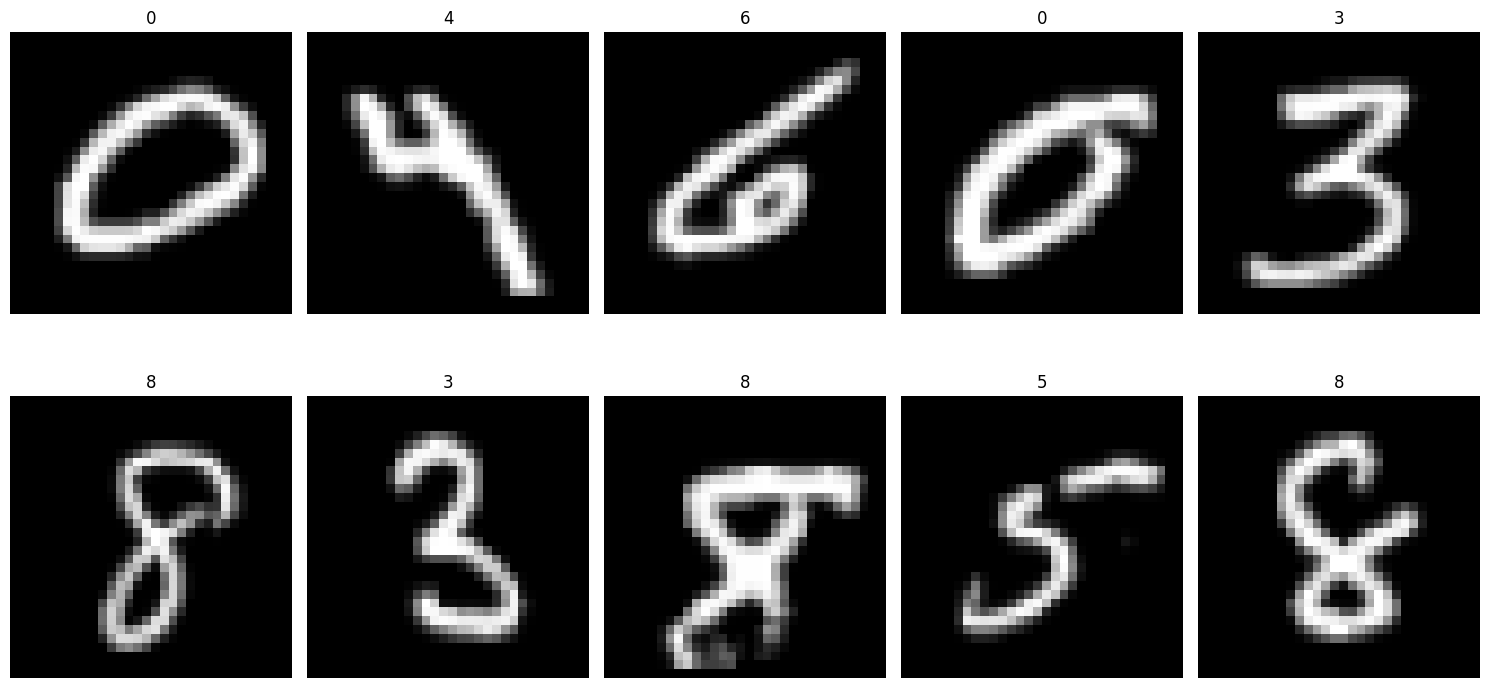
\includegraphics[width=0.75\linewidth]{Plantilla_TFG_latex//imagenes//Inf//exp/mnist.png}
    \label{fig:mnist}
    }
    \vspace{1.6cm}
    \subfloat{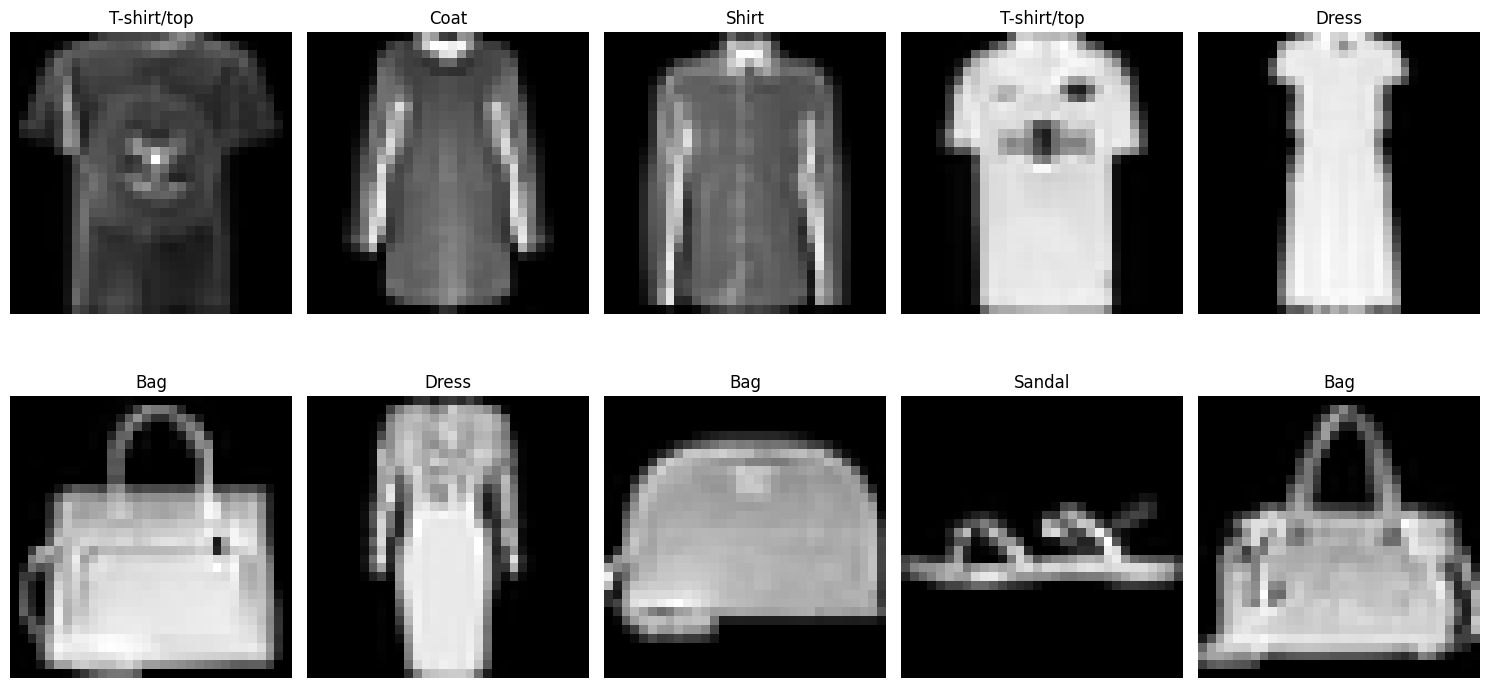
\includegraphics[width=0.75\linewidth]{Plantilla_TFG_latex//imagenes//Inf//exp/fmnist.png}
    \label{fig:fmnist}
    }
    \vspace{1.6cm}
    \subfloat{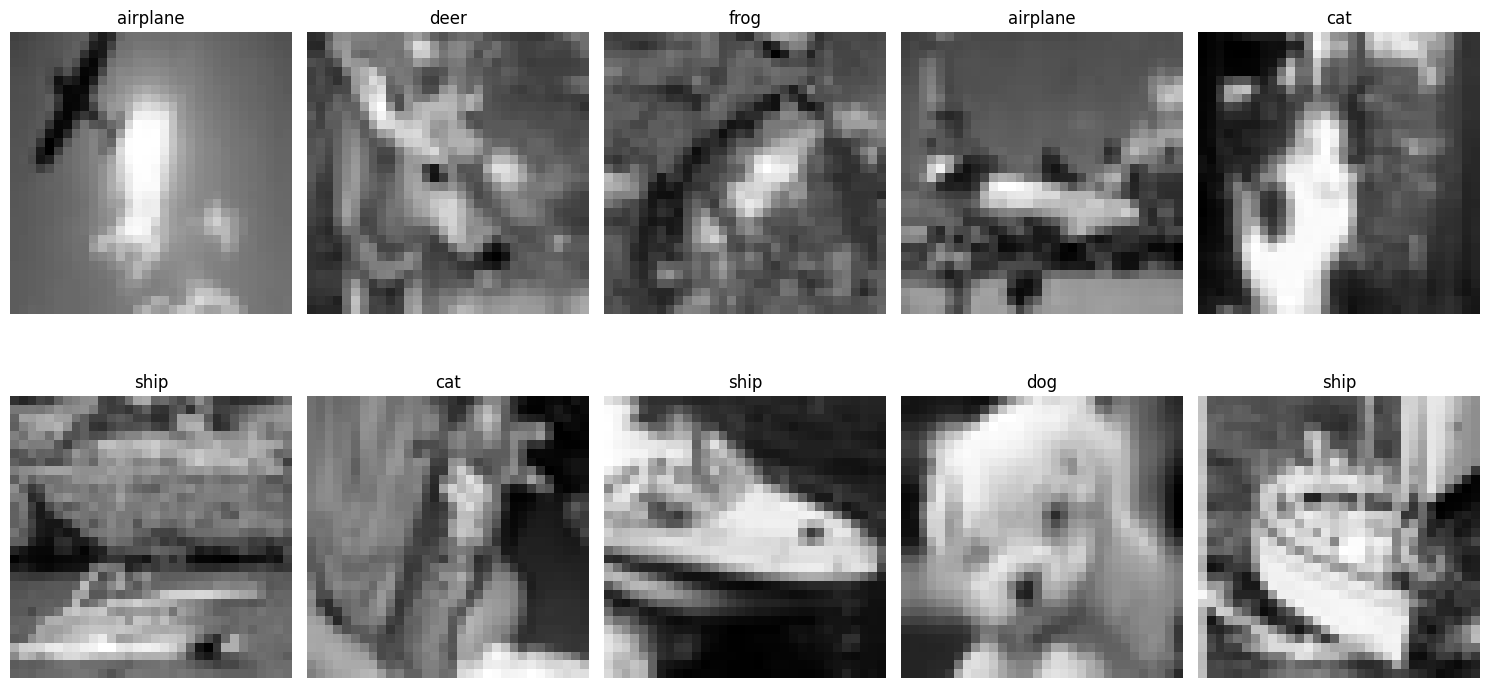
\includegraphics[width=0.75\linewidth]{Plantilla_TFG_latex//imagenes//Inf//exp/cifar10.png}
    \label{fig:cifar10}
    }
    \caption[Ejemplos de imágenes de los conjuntos de datos utilizados en la experimentación para clasificación de imágenes]{Ejemplos de imágenes de los conjuntos de datos utilizados en la experimentación para clasificación de imágenes. La primera fila (arriba) muestra muestras del conjunto MNIST, compuesto por dígitos escritos a mano en escala de grises (28×28 píxeles). La segunda fila (en medio) corresponde a Fashion-MNIST (F-MNIST), un conjunto de imágenes en escala de grises (28×28 píxeles) que representan distintos tipos de prendas de vestir y accesorios. La tercera fila (abajo) presenta ejemplos de CIFAR-10G, una versión escalada y en escala de grises (28×28 píxeles) del conjunto CIFAR-10G, que contiene imágenes de objetos como vehículos y animales. Sobre cada imagen se muestra su correspondiente etiqueta.}
\end{figure}

F-MNIST por su parte tiene imágenes en escala de grises de 10 tipos de ropa distintos (por ejemplo pantalones, camisetas, zapatos) como vemos en la Figura \ref{fig:fmnist}, con la misma resolución que MNIST pero una complejidad media-baja. Esta diferencia se debe principalmente a la mayor variabilidad en los objetos de ropa y sus características. Las imágenes son más complejas y tienen patrones más intrincados que los dígitos.


Por último CIFAR-10G contiene imágenes en resolución $32 \times 32 \times 3$, aunque las convertimos a un solo canal en escala de grises como podemos ver en la Figura \ref{fig:cifar10}, por lo que nos referimos a este conjunto de datos como CIFAR-10G. Incluye 10 clases de objetos como aviones, coches, pájaros, gatos, etc. La complejidad es alta debido a la naturaleza de las imágenes, que contienen una amplia variedad de objetos con diferentes formas, texturas y fondos. Las imágenes son relativamente pequeñas en resolución para la cantidad de información contenida en ellas, haciendo más difídil distinguir pequeños detalles necesarios para una correcta clasificación. La variabilidad en los datos requiere de técnicas más avanzadas para clasificación, haciéndolo un \textit{benchmark} estandarizado para evaluar modelos de aprendizaje profundo. Reducir las imágenes a un solo canal ayuda a reducir la cantidad de parámetros del modelo y el tiempo de entrenamiento, pero para saber si afecta a la complejidad de la tarea habría que realizar un análisis específico, ya que aunque perdemos información sobre los datos no está claro que sea información relevante. Para ello, por ejemplo, los colores deberían ser consistentes dentro de una misma clase, y diferentes a los colores de las demás.












\subsection{Modelos}
\label{sec:modelos}

Usaremos dos familias de modelos: MLP y ConvNets. Con los primeros usaremos conjuntos de datos tabulares para clasificación y regresión, y con los segundos conjuntos de datos de imágenes para la tarea de clasificación. La implementación de los MLP se ha realizado a través de la librería FastAI por simplicidad ya que ofrece lo necesario para usarlos directamente. La implementación de las ConvNets se ha realizado desde cero, observando la topología de LeNet5 y las ResNets en sus papers originales, ya que en ellas sí que se han introducido ciertos cambios que se comentan más adelante. Todos los modelos han sido entrenados desde cero.

Usaremos 4 modelos de tipo MLP, con 1,2,5 y 11 capas ocultas cada uno. El número de neuronas por capa es una potencia de 2 y con estructura piramidal incremental, es decir primero aumentando el número de neuronas por capa y luego disminuyéndolo. Estas son elecciones comunes en la literatura ya que facilitan las operaciones por su estructura (la primera) y el tratamiento de los datos (la segunda).

\begin{table}[]
\centering
\begin{tabular}{|c|c|c|}
\hline
\textbf{Capas ocultas} & \textbf{Neuronas por capa}                                                                     & \textbf{Parámetros} \\ \hline
1                      & 64                                                                                             & 2238                \\ \hline
2                      & 64, 64                                                                                         & 6462                \\ \hline
5                      & 64, 128, 256, 128, 64                                                                          & 85k                 \\ \hline
11                     & \begin{tabular}[c]{@{}c@{}}32, 64, 128, 256, 512, 1024, \\ 512, 256, 128, 64 y 32\end{tabular} & 1.4M                \\ \hline
\end{tabular}
\caption[Características de los modelos de Perceptrón Multicapa utilizados en la experimentación]{Características de los modelos MLP utilizados en la experimentación. Se detalla el número de capas ocultas, la cantidad de neuronas en cada capa oculta (en orden) y el número total de parámetros del modelo, incluyendo aquellos asociados a capas BatchNorm. Los modelos varían desde arquitecturas simples con una sola capa oculta de 64 neuronas y 2,238 parámetros, hasta arquitecturas profundas con 11 capas ocultas y 1.4 millones de parámetros, permitiendo evaluar el impacto de la profundidad en el desempeño de distintas estrategias de entrenamiento.}
\label{tab:MLPmod}
\end{table}

Antes de cada capa linal hay una capa BatchNorm1D, ya que es la implementación por defecto de FastAI y mejora el rendimiento en el entrenamiento. Los parámetros asociados a este tipo de capa van incluidos en el cómputo de la Tabla \ref{tab:MLPmod}. En caso de que la tarea sea clasificación, la librería PyTorch incluye automáticamente una capa de \textit{SoftMax} al final del modelo.

Para los modelos basados en convoluciones usamos LeNet5 y dos ResNets, con 15 y 57 capas. En el primero sustituimos las funciones de activación por ReLU, ya que en la literatura posterior a la presentación del modelo se han demostrado superiores a las sigmoides y la tangente hiperbólica. También se han sustituido las capas de \textit{AveragePool} por \textit{MaxPool} y añadido capas de BatchNorm por los mismos motivos. En la Tabla \ref{table:lenet5} se muestra la topología de este modelo, obviando las capas de \textit{Flatten} y de \textit{SoftMax}. Tiene un total de 62 mil parámetros.



\begin{table}[]
\centering
\begin{tabular}{|c|c|c|c|}
\hline
\multirow{2}{*}{\textbf{Capa}} & \multirow{2}{*}{\textbf{Dimensión}} & \multirow{2}{*}{\textbf{Kernel}} & \multirow{2}{*}{\textbf{Canales}} \\
                               &                                     &                                  &                                   \\ \hline
Convolución                    & 28x28                               & 5x5                              & 6                                 \\ \hline
BatchNorm2D                    & 28x28                               & -                                & -                                 \\ \hline
ReLU                           & 28x28                               & -                                & -                                 \\ \hline
Max Pool                       & 14x14                               & 2x2, stride 2                    & -                                 \\ \hline
Convolución                    & 10x10                               & 5x5                              & 16                                \\ \hline
BatchNorm2D                    & 10x10                               & -                                & -                                 \\ \hline
ReLU                           & 10x10                               & -                                & -                                 \\ \hline
Max Pooling                    & 5x5                                 & 2x2                              & -                                 \\ \hline
Lineal                         & 120                                 & -                                & -                                 \\ \hline
BatchNorm1D                    & 120                                 & -                                & -                                 \\ \hline
ReLU                           & 120                                 & -                                & -                                 \\ \hline
Lineal                         & 84                                  & -                                & -                                 \\ \hline
BatchNorm1D                    & 84                                  & -                                & -                                 \\ \hline
ReLU                           & 84                                  & -                                & -                                 \\ \hline
Lineal                         & num\_classes                        & -                                & -                                 \\ \hline
\end{tabular}
\caption[Arquitectura del modelo LeNet5 utilizado en la experimentación para clasificación de imágenes de 28×28 píxeles con un solo canal de entrada]{Arquitectura del modelo LeNet5 utilizado en la experimentación para clasificación de imágenes de 28×28 píxeles con un solo canal de entrada. Se detallan las capas que componen la red, incluyendo convoluciones, capas BatchNorm, activaciones ReLU, \textit{Max Pooling} y capas totalmente conectadas (Lineal). La columna ``Dimensión'' indica el tamaño espacial de la salida de cada capa, mientras que la columna ``Canales'' representa el número de mapas de características generados. En las capas lineales, la dimensión corresponde al número de neuronas.}
\label{table:lenet5}
\end{table}


Se han diseñado dos modelos de ResNet, uno con 15 capas y otro con 57. Los bloques convolucionales agrupan 3 capas de convolución con sus respectivas capas BatchNorm, y se usan convoluciones 1x1 para hacer cuello de botella, reduciendo así el número de parámetros sin perder expresividad de la red. Se sigue el diseño usual de esta familia de modelos, por ejemplo agrupando más bloques convolucionales en mitad de la red, con una convolución previa a los bloques convolucionales y usando solo una capa lineal. El modelo ResNet57 que se implementa tiene un total de 1.3M de parámetros, mientras que ResNet15 tiene 500 mil. Sus topologías pueden observarse en la Tabla \ref{table:resnet57} y la Tabla \ref{table:resnet15} respectivamente. 

\begin{table}[]
\begin{tabular}{|c|c|c|c|}
\hline
\multirow{2}{*}{\textbf{Capa}} & \multirow{2}{*}{\textbf{Dimensión}} & \multirow{2}{*}{\textbf{Kernel/Stride}} & \multirow{2}{*}{\textbf{Canales}} \\
                               &                                            &                                         &                                          \\ \hline
Convolución                    & 26x26                                      & 7x7                                     & 64                                       \\ \hline
BatchNorm2d                    & 26x26                                      & -                                       & -                                        \\ \hline
ReLU                           & 26x26                                      & -                                       & -                                        \\ \hline
MaxPool2d                      & 13x13                                      & 2x2, stride 2, padding 1                & -                                        \\ \hline
BottleneckBlock x3             & 13x13                                      & 1x1, 3x3, 1x1                           & 64                                       \\ \hline
BottleneckBlock x4             & 7x7                                        & 1x1, 3x3, 1x1, stride 2                 & 128                                      \\ \hline
BottleneckBlock x4             & 4x4                                        & 1x1, 3x3, 1x1, stride 2                 & 256                                      \\ \hline
BottleneckBlock x3             & 2x2                                        & 1x1, 3x3, 1x1, stride 2                 & 512                                      \\ \hline
AdaptiveAvgPool2d              & 512                                        & -                                       & -                                        \\ \hline
BatchNorm1d                    & 512                                        & -                                       & -                                        \\ \hline
Dropout                        & 512                                        & -                                       & -                                        \\ \hline
Lineal                         & num\_classes                               & -                                       & -                                        \\ \hline
\end{tabular}
\caption[Arquitectura del modelo ResNet57 utilizado en la experimentación para clasificación de imágenes de 28×28 píxeles con un solo canal de entrada]{Arquitectura del modelo ResNet57 utilizado en la experimentación para clasificación de imágenes de 28×28 píxeles con un solo canal de entrada. La tabla describe la secuencia de capas de la red, incluyendo convoluciones iniciales, capas BatchNorm, activaciones ReLU, \textit{MaxPool}, bloques residuales tipo Bottleneck, \textit{AdaptiveAvgPool}, regularización mediante \textit{Dropout} y una capa lineal final. La columna ``Dimensión'' indica el tamaño espacial de la salida de cada capa, mientras que la columna ``Canales'' representa el número de mapas de características generados. En las capas lineales, la dimensión corresponde al número de neuronas.}
\label{table:resnet57}
\end{table}


\begin{table}[]
\begin{tabular}{|c|c|c|c|}
\hline
\multirow{2}{*}{\textbf{Capa}} & \multirow{2}{*}{\textbf{Dimensión}} & \multirow{2}{*}{\textbf{Kernel/Stride}} & \multirow{2}{*}{\textbf{Canales}} \\
                               &                                     &                                         &                                   \\ \hline
Convolución                    & 26x26                               & 7x7                                     & 64                                \\ \hline
BatchNorm2d                    & 26x26                               & -                                       & -                                 \\ \hline
ReLU                           & 26x26                               & -                                       & -                                 \\ \hline
MaxPool2d                      & 13x13                               & 2x2, stride 2, padding 1                & -                                 \\ \hline
BottleneckBlock x1             & 13x13                               & 1x1, 3x3, 1x1                           & 64                                \\ \hline
BottleneckBlock x1             & 7x7                                 & 1x1, 3x3, 1x1, stride 2                 & 128                               \\ \hline
BottleneckBlock x1             & 4x4                                 & 1x1, 3x3, 1x1, stride 2                 & 256                               \\ \hline
BottleneckBlock x1             & 2x2                                 & 1x1, 3x3, 1x1, stride 2                 & 512                               \\ \hline
AdaptiveAvgPool2d              & 512                                 & -                                       & -                                 \\ \hline
BatchNorm1d                    & 512                                 & -                                       & -                                 \\ \hline
Dropout                        & 512                                 & -                                       & -                                 \\ \hline
Lineal                         & num\_classes                        & -                                       & -                                 \\ \hline
\end{tabular}
\caption[Arquitectura del modelo ResNet15 utilizado en la experimentación para clasificación de imágenes de 28x28 píxeles con un solo canal de entrada]{Arquitectura del modelo ResNet15 utilizado en la experimentación para clasificación de imágenes de 28x28 píxeles con un solo canal de entrada. Se detallan las capas de la red, incluyendo convoluciones, capas BatchNorm, activaciones ReLU, agrupamiento máximo (MaxPool), bloques tipo Bottleneck, agrupamiento adaptativo promedio (AdaptiveAvgPool), regularización mediante Dropout y una capa lineal final. La columna "Dimensión" indica el tamaño espacial de la salida de cada capa, mientras que la columna "Canales" representa el número de mapas de características generados. En las capas lineales, la dimensión corresponde al número de neuronas.}
\label{table:resnet15}
\end{table}





